\documentclass[xcolor=dvipsnames]{beamer}
\usepackage[UTF8,scheme=plain]{ctex}
\usepackage{hyperref}
	\def\MR#1{\href{http://www.ams.org/mathscinet-getitem?mr=#1}{MR-#1}}
	\def\ARXIV#1{\href{https://arxiv.org/abs/#1}{arXiv:#1}}
\usepackage{lmodern}
\usepackage{mathrsfs}
\usepackage{graphicx}
\usepackage[export]{adjustbox}
\usepackage{comment}
\usepackage{mathtools}
\mathtoolsset{showonlyrefs}
\usetheme{Madrid}
\usecolortheme{seahorse}
\usecolortheme{rose}
\usefonttheme{serif}
\usefonttheme{structurebold}
\setbeamerfont{title}{shape=\itshape,family=\rmfamily}
\setbeamercolor{title}{fg=red!80!black,bg=red!20!white}
%---Top matter---
\title[]{临界分支过程与超过程的脊柱分解与极限定理}
%\subtitle{Optional Subtitle}
\author[]{\textbf{孙振尧}}
\date{2019年5月}
\institute[]{
导师:任艳霞\\
合作导师:宋仁明\\
北京大学,博士生论文答辩\\
}
\begin{document}

%---Document body--------
\begin{frame}
  \titlepage
\end{frame}

%---Top matter---------
\title[]{Spine decompositions and limit theorems for critical branching processes and critical superprocesses}
\author[]{\textbf{Zhenyao Sun}}
\institute[]{
Advisor: Yan-Xia Ren\\
Co-advisor: Renming Song\\
Peking University, PhD Dissertation Defense}
\date{May, 2019}


\begin{frame}
\titlepage
\end{frame}

\begin{frame}
\frametitle{Outline}
\tableofcontents
\end{frame}
\section{Background}
\subsection{Limit theorems for critical branching processes}
\begin{frame}{Background: Kolmogorov's result}
  \begin{theorem}[Kesten, Ney and Spitzer (1966)]
Let $(Z_n)_{n\in \mathbb N}$ be a critical Galton-Watson process with offspring variance $\sigma^2 \in (0,\infty)$. 
Then
\begin{align}
n P(Z_n > 0) \xrightarrow[n\to \infty]{} \frac{2}{\sigma^2}.
\end{align}
\end{theorem}
\begin{itemize}
\item
Kolmogorov (1938) obtained the above Theorem under a three moment condition.
\end{itemize}
\end{frame}

\begin{frame}{Background: Yaglom's result}
\begin{theorem}[Kesten, Ney and Spitzer (1966)]
Let $(Z_n)_{n\in \mathbb N}$ be a critical Galton-Watson process with offspring variance $\sigma^2 \in (0,\infty)$.
Then 
\begin{align}
  \left\{ \frac{Z_n}{n}; P(\cdot | Z_n > 0) \right\} 
\xrightarrow[n\to \infty]{d} \frac{\sigma^2}{2} {\color{red} \mathbf e},
\end{align}
where {\color{red} $\mathbf e$} is an exponential random variable with mean $1$.
\end{theorem}
\begin{itemize}
\item
Yaglom (1947) obtained the above Theorem under a stronger condition.
\end{itemize}
\end{frame}

\begin{frame}{Background: Slack's result}
\begin{theorem}[Slack (1968)]
	Let $(Z_n)_{n\geq 0}$ be a critical Galton-Watson process with offspring generating function
$
	f(s)
	= s + (1-s)^{\alpha} l(1-s)
$
  where $\alpha \in (1,2]$ and $l$ is a slowly varing function at $0$.
  Then
$
	P(Z_n > 0) = n^{-1/(\alpha-1)} L(n)
$ 
where $L$ is slowly varying at $\infty$;
 and
\[
  \big\{ P(Z_n > 0) Z_n; P(\cdot | Z_n > 0)\big\}
	\xrightarrow[n\to \infty]{d} {\color{red}\mathbf z^{(\alpha-1)} },
\]
	where {\color{red} $\mathbf z^{(\alpha-1)}$} is a positive random variable with Laplace transform
\[
	E[e^{- u {\color{red} \mathbf z^{(\alpha-1)}} } ]
	= 1 - (1+ u^{-(\alpha-1)})^{-1/(\alpha-1)},
	\quad u \geq 0.
\]
\end{theorem}
\begin{itemize}
\item
  Zolotarev (1957) obtained the above Theorem under a stronger condition.
\end{itemize}
\end{frame}

\begin{frame}
\begin{table}[] 
\resizebox{\textwidth}{!}{%
\begin{tabular}{|l|l|l|l|}
\hline
 &  $\alpha = 2$: Analytical & $\alpha = 2$: Probabilistic & $\alpha \in (1,2)$ \\ \hline
  \begin{tabular}[c]{@{}l@{}} Galton-Watson \\ (GW) processes \end{tabular} & \begin{tabular}[c]{@{}l@{}} Kolmogorov (1938)\\ Yaglom (1947)\\ Kesten, Ney \\ and Spitzer (1966) \end{tabular} & \begin{tabular}[c]{@{}l@{}} Lyons, Pemantle \\ and Peres (1995)\\ Geiger (1999) \\ Geiger (2000)\\ {\color{red} Ren, Song} \\ {\color{red} and Sun (2018)}\end{tabular} & \begin{tabular}[c]{@{}l@{}} Zolotarev (1957)\\ Slack (1968)\end{tabular} \\ \hline
  \begin{tabular}[c]{@{}l@{}} Multitype GW \end{tabular} & \begin{tabular}[c]{@{}l@{}} Joffe and Spitzer \\ (1967)\end{tabular} & \begin{tabular}[c]{@{}l@{}} Vatutin and \\ Dyakonova (2001)\end{tabular} & \begin{tabular}[c]{@{}l@{}} Goldstein and Hoppe \\ (1978)\end{tabular} \\ \hline
\begin{tabular}[c]{@{}l@{}} Continuous time \\ GW process \end{tabular} & \begin{tabular}[c]{@{}l@{}} Athreya and Ney \\ (1972)\end{tabular} & - & Vatutin (1977) \\ \hline
\begin{tabular}[c]{@{}l@{}} Continuous time \\ Multitype \\ GW process \end{tabular} & \begin{tabular}[c]{@{}l@{}} Athreya and Ney\\ (1974)\end{tabular} & - & Vatutin (1977) \\ \hline
\begin{tabular}[c]{@{}l@{}} Branching Markov \\ processes \end{tabular} & \begin{tabular}[c]{@{}l@{}} Asmussen and \\ Hering (1983)\end{tabular} & Powell (2015) & \begin{tabular}[c]{@{}l@{}} Asmussen and Hering \\ (1983)\end{tabular} \\ \hline
  \begin{tabular}[c]{@{}l@{}} Continuous-state \\ branching processes \end{tabular} & \begin{tabular}[c]{@{}l@{}} Li (2000)\\ Lambert (2007)\end{tabular} & \begin{tabular}[c]{@{}l@{}} {\color{red} Ren, Song} \\ {\color{red} and Sun (2019)}\end{tabular} & \begin{tabular}[c]{@{}l@{}} Kyprianou and Pardo \\ (2008)\\ Ren, Yang \\ and Zhao (2014)\end{tabular} \\ \hline
Superprocesses & \begin{tabular}[c]{@{}l@{}} Evans and Perkins (1990) \\ Ren, Song \\ and Zhang (2015)\end{tabular} & \begin{tabular}[c]{@{}l@{}} {\color{red} Ren, Song} \\ {\color{red} and Sun (2019)}\end{tabular} & \begin{tabular}[c]{@{}l@{}} {\color{red} Ren, Song} \\ {\color{red} and Sun (2019+)}\end{tabular} \\ \hline
\end{tabular}%
}
\end{table} 
\end{frame}
\section{Model}
\subsection{Superprocesses}

\begin{frame}{Model: Settings}
\begin{itemize}
\item
  {\color{red}$E$} be a locally compact separable metric space;
\item
  {\color{red} $\mathcal M$} be the collection of all the finite Borel measures on $E$; 
\item
  Spatial motion {\color{red} $\{(\xi_t)_{t\geq 0}; (\Pi_x)_{x\in E}\}$} be an $E$-valued Hunt process with transition semigroup {\color{red} $(P_t)_{t\geq 0}$};
\item
  Branching mechanism {\color{red} $\psi$} be a function from $E\times [0,\infty)$ to $[0,\infty)$ s.t.
\[
  \psi(x,z) 
  := -\beta(x)z+\alpha(x)z^2 +\int_{(0,\infty)}(e^{-zy}-1+zy)\pi(x,dy),
\]
	where $\beta$ is a bounded measurable function on $E$, $\alpha$ is a bounded non-negative measurable function on $E$, and $\pi$ is a kernel from $E$ to $(0,\infty)$ s.t. 
\[
 \sup_{x\in E} \int_{(0,\infty)}(y\wedge y^2)\pi(x,dy)<\infty.
\] 
\end{itemize}
\end{frame}

\begin{frame}{Model: Superprocesses}
\begin{itemize}
\item
For each measure $\mu$ and function $f$, write
$\mu(f) : = \int f d\mu$ whenever the integral make sense.
\item
We say a measurable function $f$ on $\mathbb R_+ \times E$ is {\color{blue} locally bounded} if
\begin{align}
\sup_{s\in [0,t], x\in E} |f(s,x)| < \infty, \quad t\in \mathbb R_+.
\end{align}
\end{itemize}
\begin{definition}[Superprocesses]
An $\mathcal M$-valued Markov process {\color{red} $\{(X_t)_{t\geq 0}; (\mathbf P_\mu)_{\mu\in \mathcal M}\}$} is called a $(\xi,\psi)$-superprocess if for each $\mu \in \mathcal M, f\in b\mathscr B_+$ and $t\geq 0$ we have
\[
  \mathbf P_\mu [e^{-X_t(f)}] = e^{-\mu( {\color{red} V_tf} )}.
\]
Here, $(t,x) \mapsto {\color{red} V_tf(x)}$ on $[0,\infty) \times E$ is the unique {\color{blue} locally bounded} positive solution to the equation
\begin{align*}\label{eq:FKPP_in_definition}
  {\color{red} V_tf(x)} + \int_0^{t} P_{t-s} \psi \big(\cdot, {\color{red} V_sf(\cdot)}\big) (x) ds 
  = P_t f(x).
\end{align*}
\end{definition}
\end{frame}
\begin{comment}
\begin{frame}{Model: Superprocesses}
\begin{itemize}
\item
\end{itemize}
\begin{example}
  Consider a Branching Brownian motion with
\begin{itemize}
\item
  {\color{red} $k$} initial particles;
\item
  killing rate {\color{red} $2k$};
\item
  critical binary branching.
\end{itemize}
Denote by $X^{({\color{red} k})}_t(A)$ the number of particles the Borel set $A$ at time $t$. Then
\[
	\Big(\frac{1}{\color{red} k} X^{({\color{red} k})}_t(\cdot)\Big)_{t\geq 0}
	\xrightarrow[{\color{red}k}\to \infty]{d} (\xi,\Psi)\text{-superprocess}
\]
	with $\xi$ being a Brownian motion and $\Psi(z) = z^2$.
\end{example}
\end{frame}
\end{comment}
\section{Assumptions}

\begin{frame}{Model: Assumptions}
\begin{itemize}
\item
  Superprocess is the high-density limits of branching particle systems. (Watanabe (1968), Dawson (1975), Dynkin (1991)).
\item
The mean semigroup of the superprocess:
\[
\mathbf P_{\delta_x} [X_t(f)] = {\color{red} P_t^\beta} f(x) := \Pi_x[e^{\int_0^{t} \beta (\xi_r) dr}f(\xi_t)].
\]
\end{itemize}
\begin{block}{Assumption 1.}   
  There exist a $\sigma$-finite measure {\color{red} $m$} with full support on $E$ and a family of strictly positive,
	bounded continuous functions $\{ p_t(\cdot,\cdot): t > 0 \}$ on $E \times E$ such that
\begin{itemize}
\item $P_tf(x)= \int_E p_t(x,y) f(y) m(dy);$
\item $\int_E p_t(y,x)m(dy) \leq 1;$
\item $\int_E \int_E p_t(x,y)^2 m(dx) m(dy)
	<\infty;$
\item
	$x \mapsto \int_E p_t(x,y)^2 m(dy)$ and $x \mapsto \int_E p_t(y,x)^2 m(dy)$ are both continuous.
\end{itemize}
\end{block}
\end{frame}

\begin{frame}{Assumptions}
Under Assumption 1, we can say the following:
\begin{itemize}
\item
$(P^\beta_t)_{t \geq 0}$ and its disjoint $(P^{\beta *}_t)_{t \geq 0}$ are strongly continuous semigroups of compact operators in $L^2(E,m)$.
\item
Let $L$ and $L^*$ be the generators of $(P^\beta_t)_{t \geq 0}$ and $(P^{\beta *}_t)_{t \geq 0}$, respectively. 
Then ${\color{red} \lambda} := \sup \text{Re}(\sigma(L)) = \sup \text{Re}(\sigma(L^*))$ is a common {\color{red}eigenvalue} of multiplicity $1$ for both $L$ and $L^*$.
\item
The corresponding {\color{red}eigenfunctions} {\color{red} $\phi$} of $L$ and {\color{red} $\phi^*$} of $L^*$ can be chosen to be strictly positive and continuous everywhere on $E$.
\item
Normalize $\phi$ and $\phi^*$ by $\langle\phi, \phi\rangle_m = \langle\phi,\phi^*\rangle_m = 1$ so that they are unique.
\item
Operator $P_t^\beta$ has transition density {\color{red}$p_t^\beta(x,y)$} with respect to measure $m$.
\end{itemize}
\end{frame}

\begin{frame}{Assumptions}

\begin{block}{Assumption 2 (Critical and Intrinsic Ultracontractive)}
  \begin{itemize}
  \item 
    $\lambda = 0$.
  \item
    $\forall t > 0, \exists c_t>0, \forall x,y \in E, \quad p_t^\beta (x,y) \leq c_t \phi(x) \phi^*(y)$.
  \end{itemize}
\end{block}
Under Assumption 2, the following are true
\begin{itemize}
\item for each $\mu \in \mathcal M$, we have $\mathbf P_\mu [X_t(\phi)] = \mu(\phi)$;
\item there exists $c,\rho > 0$ such that for all $t > 1$,
  \begin{align}
    \sup_{x,y \in E} \left| \frac{p^\beta_t(x,y)}{ \phi(x) \phi^*(y)} - 1 \right| 
\leq ce^{-\rho t}.
  \end{align}
\end{itemize}
\end{frame}

\section{Results}
\subsection{Kolmogorov type result}
\subsection{Yaglom type result}
\subsection{Slack type result}

\begin{frame}{Model: Assumptions}
  \begin{block}{Assumption 3 (Non-persistence and second moment condition)}
    \begin{itemize}
    \item 
      $\forall x \in E, t > 0, \quad \mathbf P_{\delta_x} ( X_t(1) = 0) > 0$.
    \item
      Define 	$\nu(dx) : = \phi^* (x) m(dx)$, then $\mathbf P_\nu(X_t(1) = 0) > 0$ for some $t>0$.
    \item
      Define $A(x):= 2\alpha(x) + \int_{(0,\infty)} y^2\pi(x,dy)$, then $\|A\cdot \phi\|_\infty < \infty$.
    \end{itemize}
  \end{block}
\end{frame}

\begin{frame}{Kolmogorov type and Yaglom type results}
\begin{block}{Theorem. 1}
Suppose that Assumptions 1, 2 and 3 hold. 
Then for each $\mu \in \mathcal M$ with $\mu(\phi)<\infty$, we have
	\[
	t\mathbf P_\mu\left(\|X_t\| > 0\right)
	\xrightarrow[t\to\infty]{} \frac{\mu(\phi)} {\frac{1}{2}\langle  A \phi,\phi \phi^*\rangle_m}.
	\]
Furthermore, for each non-negative measurable function $f$ with $\|\phi^{-1}f\|_\infty < \infty$, we have
	\[\begin{split}
	\left\{t^{-1}X_t(f);\mathbf P_\mu\left(\cdot \middle| \| X_t\| > 0\right)\right\}
	\xrightarrow[t\to\infty]{d} \frac{1}{2}\langle \phi^*, f\rangle_m\langle A\phi, \phi\phi^*\rangle_m \mathbf e,
	\end{split}\]
	where $\mathbf e$ is an exponential random variable with mean 1.
\end{block}
\end{frame}

\begin{frame}{Remark}
\begin{itemize}
\item
Ren, Song and Zhang (2015) obtained the above result under a slightly stronger condition.
\item
Ren, Song and Zhang (2015)'s approach is more analytical while our approach is more probabilistic.
\item
We characterized some measure transform of the superprocesses.
\end{itemize}
\begin{definition}[Size-biased transform]
Let $G$ be a non-negative measurable function which is integrable with respect to a $\sigma$-finite measure $Q$.
A probability measure {\color{red} $Q^G$} is called the $G$-transform of $Q$ if
  \[
    d{\color{red} Q^G} = \frac{G}{Q[G]} dQ.
  \]
\end{definition}
\end{frame}

\begin{frame}{Remark: Probabilistic approach}
\begin{block}{Lemma}
Let $\mathcal N$ be a Poisson random measure with intensity measure $N$. 
Let $F$ be a non-negative testing function with $0 < N[F] < \infty$.
Then    
\[
      \{\mathcal N; P^{\mathcal N(F)}\}
      \overset{d}{=} \{\mathcal N ; P\} \otimes \{ \delta_s; N^F(ds)\}.
\]
\end{block}
  \begin{figure}[h]
    \begin{tabular}{ll}
      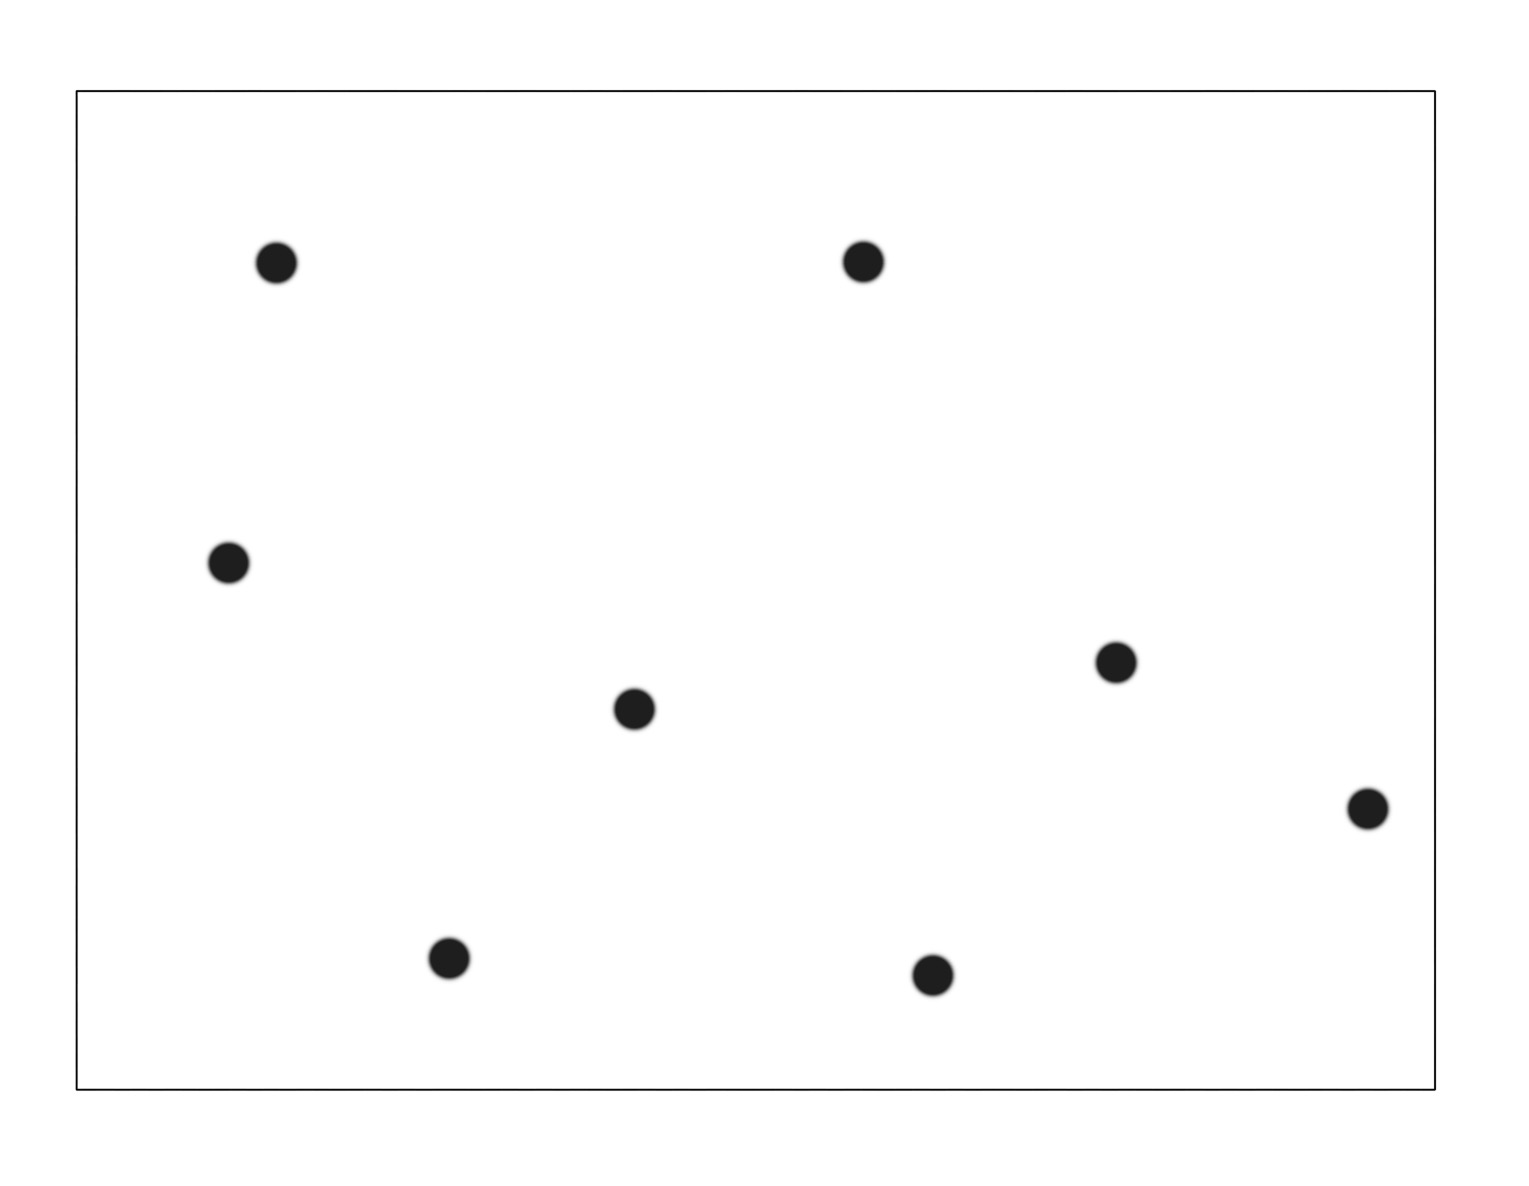
\includegraphics[scale=0.08]{001.jpg}
      &
        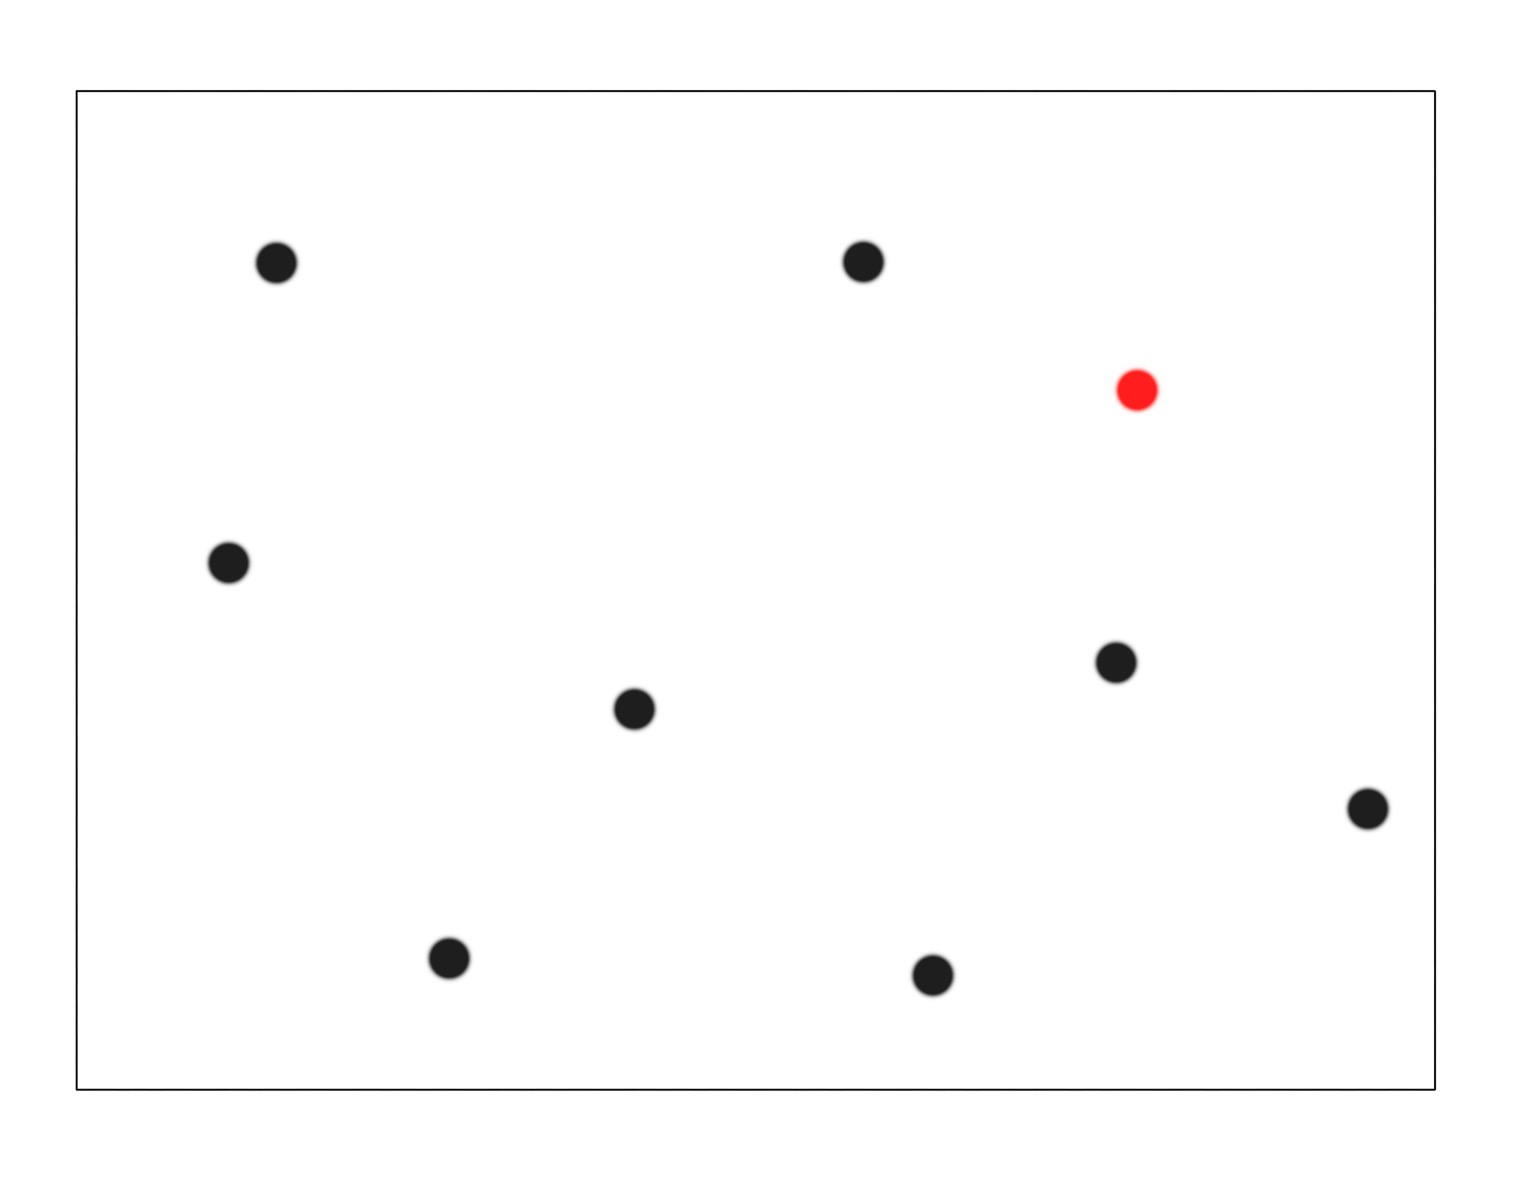
\includegraphics[scale=0.08]{002.jpg}
    \end{tabular}
  \end{figure}
\end{frame}


\begin{frame}{Remark: Probabilistic approach}
\begin{itemize}
\item
  The {\color{red} Kuznetsov measures $(\mathbb N_x)_{x\in E}$} of superprocess $(X_t)_{t\geq 0}$ is given by the following Theorem:
\end{itemize}
  \begin{theorem}[Li (2011) Theorem 8.24]
There is a family of $\sigma$-finite measures {\color{red} $(\mathbb N_x)_{x\in E}$} on space
\begin{align}
  \mathbb D &:= \{\mathcal M\text{-valued c\`adl\`ag functions on $[0,\infty)$} 
\\ &\qquad \text{with the null measure as a trap}\} 
\end{align}
such that for each $x\in E$, 
\begin{align}
\{(X_t)_{t>0}; \mathbf P_{\delta_x} \}
  \overset{d}{=} \left( \int_{\mathbb D} w_t \mathcal N(dw) \right)_{t>0},
\end{align}
where {\color{red} $\mathcal N$} is a Poisson random measure on $\mathbb D$ with intensity measure {\color{red} $\mathbb N_x$}.
\end{theorem}
\end{frame}

\begin{frame}{Remark: Probabilistic approach}
\begin{itemize}
\item 
Let $\mu \in \mathcal M$ and write $\mathbb N_\mu(\cdot) := \int_{E} \mathbb N_x(\cdot)\mu(dx)$.
\end{itemize}
\begin{block}{Theorem 2.}
For each non-negative measurable function $F$ on $\mathbb D$ with $\mathbb N_\mu[F] \in (0,\infty)$, we have 
\begin{align}
\{(X_t)_{t\geq 0}; \mathbf P^{\mathcal N(F)}_\mu\} 
\overset{d}{=} \{(X_t)_{t\geq 0}; \mathbf P_\mu\} \otimes \{(w_t)_{t \geq 0}; \mathbb N^F_\mu(dw)\}.
\end{align}
\end{block}
    We can characterize $\{(w_t)_{t \geq 0}; \mathbb N^F_\mu(dw)\}$ while
    \begin{itemize}
    \item 
      $F(w) = w_t(\phi)$ using the {\color{blue} classical Spine Decomposition Theorem}.
    \item 
      $F(w) = w_t(f)$ using a {\color{red} generalized Spine Decomposition Theorem}.
    \item 
      $F(w) = w_t(\phi)^2$ using a {\color{red} 2-Spine Decomposition Theorem.}
    \end{itemize}
\end{frame}


\begin{frame}{Remark: Probabilistic approach}
\begin{itemize}
\item
{\color{blue} The classical Spine Decomposition Theorem} is developed in Engl\"ander and kyprianou (2004) and Liu, Ren and Song (2009), and Eckhoff, Kyprianou and Winkel (2015).
\item
{\color{red} The 2-Spine Decomposition Theorem} for superprocesses 
\begin{itemize}
\item
is an analog of the two-spine decomposition theorem for \textbf{Galton-Watson trees} in Ren, Song and Sun (2018), 
\item
and is related to the \textbf{multi-spine theory} appeared in Harris and Roberts (2017) in the context of \textbf{branching Markov process}, 
\item
and is closely related to Harris, Johnston and Roberts (arXiv), Johnston (arXiv) and Abraham and Pierre (arXiv) in the context of \textbf{Galton-Watson trees}.
\end{itemize}
\end{itemize}
\end{frame}

\begin{frame}{Model: Without the second moment condition}
\begin{itemize}
\item We now consider a superprocess $(X_t)_{t\geq 0}$ which satisfies Assumptions 1, 2 and the following: 
\end{itemize}
\begin{block}{Assumption 4 (Stable branching)}
  The branching mechanism $\psi$ is of the form:
\begin{align*}
  \psi(x,z)
  = -\beta (x) z + \kappa(x) z^{\gamma(x)},
\end{align*}
  where $\beta \in \mathscr B_b(E), \gamma \in \mathscr B^+_b(E)$, $\kappa \in \mathscr B^+_b(E)$ with $1< \gamma(\cdot )<2$. 
We also assume that 
\[{\color{red} \gamma_0} := \operatorname{ess\,inf}_{m(dx)} \gamma(x)> 1\] and $\kappa_0:=\operatorname{ess\,inf}_{m(dx)}\kappa(x) > 0$.
\end{block}
\end{frame}

\section{Remarks}
\begin{frame}{Results: Slack type}
\begin{block}{Theorem 3}
Under Assumptions 1,2 and 4, we have
\begin{itemize}
\item[(1)]
  $\mathbf P_{\delta_x}( \| X_t\| = 0) > 0$, for each $t > 0$ and $x\in E$.
\item[(2)]
  For each $\mu \in \mathcal M$, $\mathbf P_{\mu}(\|X_t\| \neq 0) = {\color{red} t^{-\frac{1}{\gamma_0 - 1}}} L(t)$ where $L(t)$ is a slowly varing function at $\infty$.
\end{itemize}
Write $C_X := \langle \mathbf 1_{\gamma(\cdot) = {\color{red} \gamma_0}} \kappa\cdot \phi^{ \color{red} \gamma_0}, \phi^* \rangle_m$ and $\eta_t := \big( C_X(\gamma_0 - 1) {\color{red} t} \big)^{\color{red} - 1/(\gamma_0 - 1) }$. 
{\color{red} Further assume} that $m( x:\gamma(x)={\color{red}\gamma_0} )>0$, then
\begin{itemize}
\item[(3)]
$
  \lim_{t\to\infty} \eta_t^{-1}\mathbf P_{\mu}(\|X_t\| \neq 0)
  =\mu(\phi);
$
\item[(4)]
  for each $f \in \mathscr B^+(E)$ with $\langle f, \phi^* \rangle_m > 0$ and $\| \phi^{-1}f \|_\infty < \infty$,
\[
  \{\eta_t X_t(f) ; \mathbf P_{\mu}(\cdot |\|X_t\| \neq 0) \}
  \xrightarrow[t\to \infty]{d} \langle f, \phi^*\rangle_m {\color{red}\mathbf z^{(\gamma_0 - 1)}}.
\]
\end{itemize}
\end{block}
\end{frame}

\begin{frame}{Remark: Slack type result}
\begin{itemize}
\item
{\color{red} The asymptotic behavior} of the critical superprocesses with spatially dependent stable branching {\color{red} is dominated by the heaviest tail $\gamma_0$}.
\item
The weak limit is {\color{red} universal}: the distribution of $\mathbf z^{(\gamma_0 - 1)}$ is only related to $\gamma_0$.
\item
We used the {\color{red} generalized Spine Decomposition Theorem} to establish the Slack type result.
\item
We also used an {\color{red} analytical argument} which can be considered as the {\color{red} analytical alternative} to the {\color{red} 2-spine Decomposition Theorem}.
\end{itemize}
\end{frame}
\begin{frame}{Other Results}
In Chapter 2, we established a {\color{red} 2-Spine Decomposition Theorem} for the {\color{red} critical Galton-Watson trees} to characterize its $Z_n(Z_n - 1)$-transform.
\begin{figure}[h]
  \begin{tabular}{ll}
    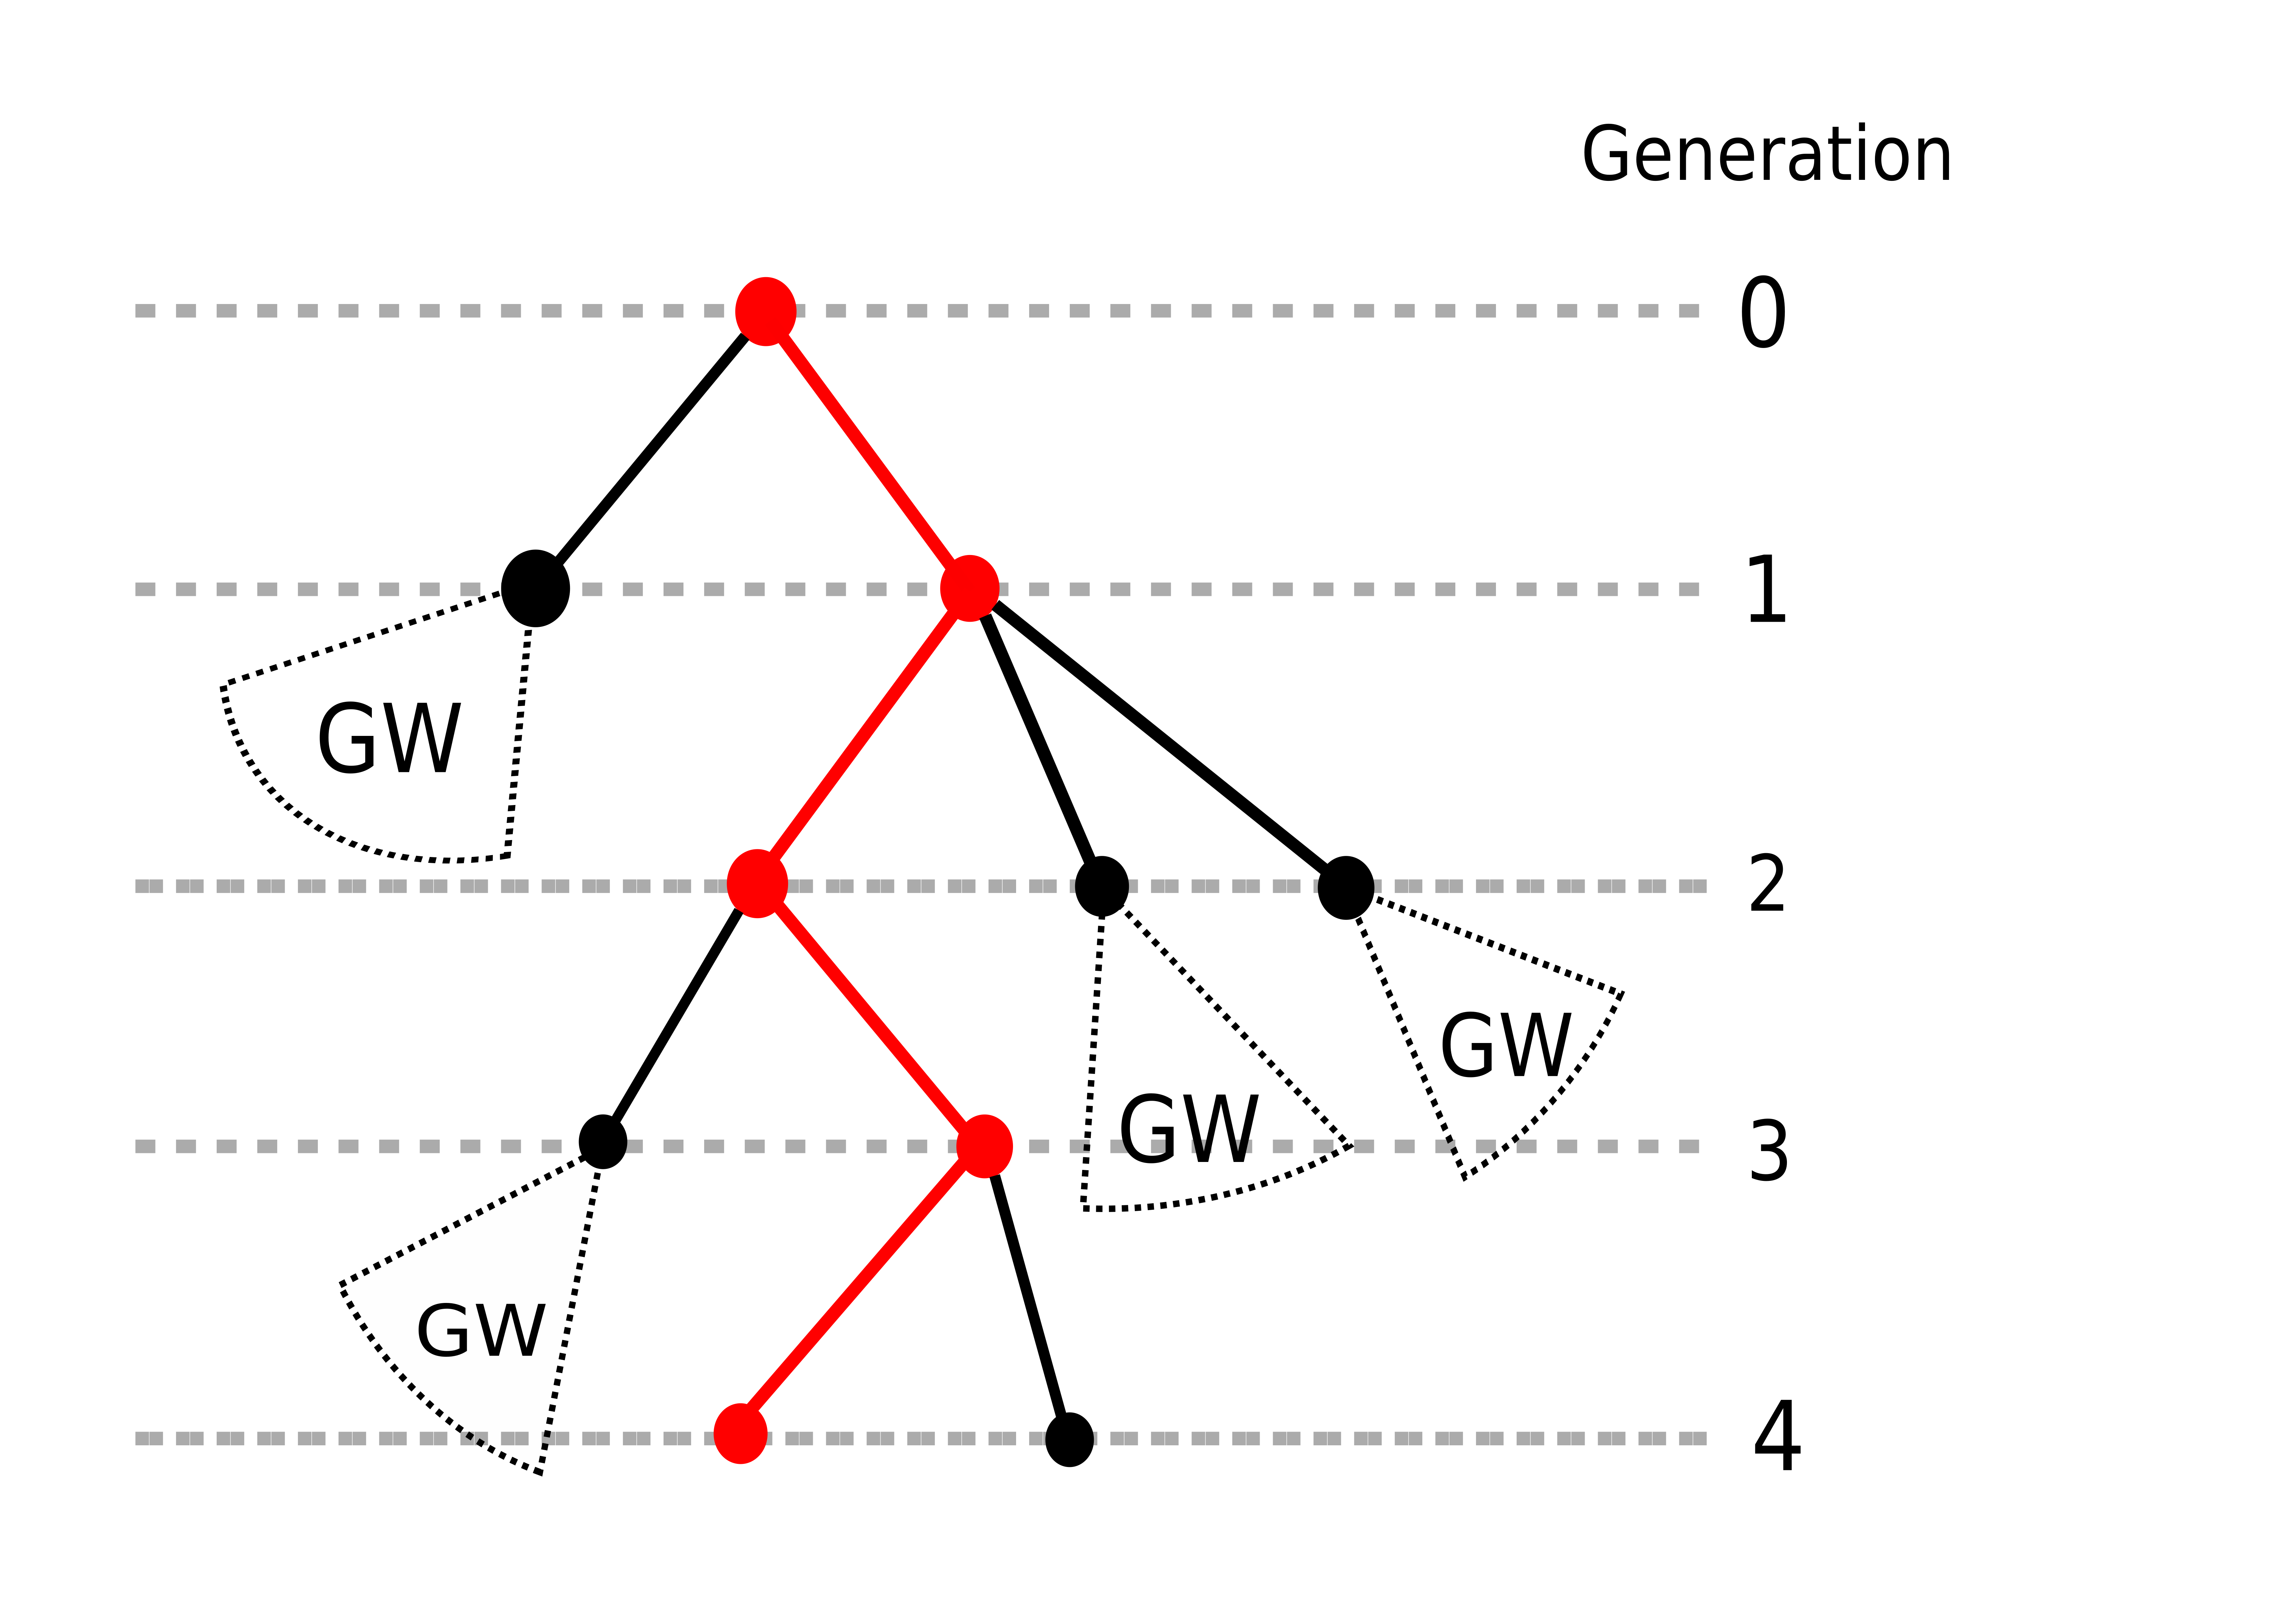
\includegraphics[scale=0.35]{1-spine.png}
    &
      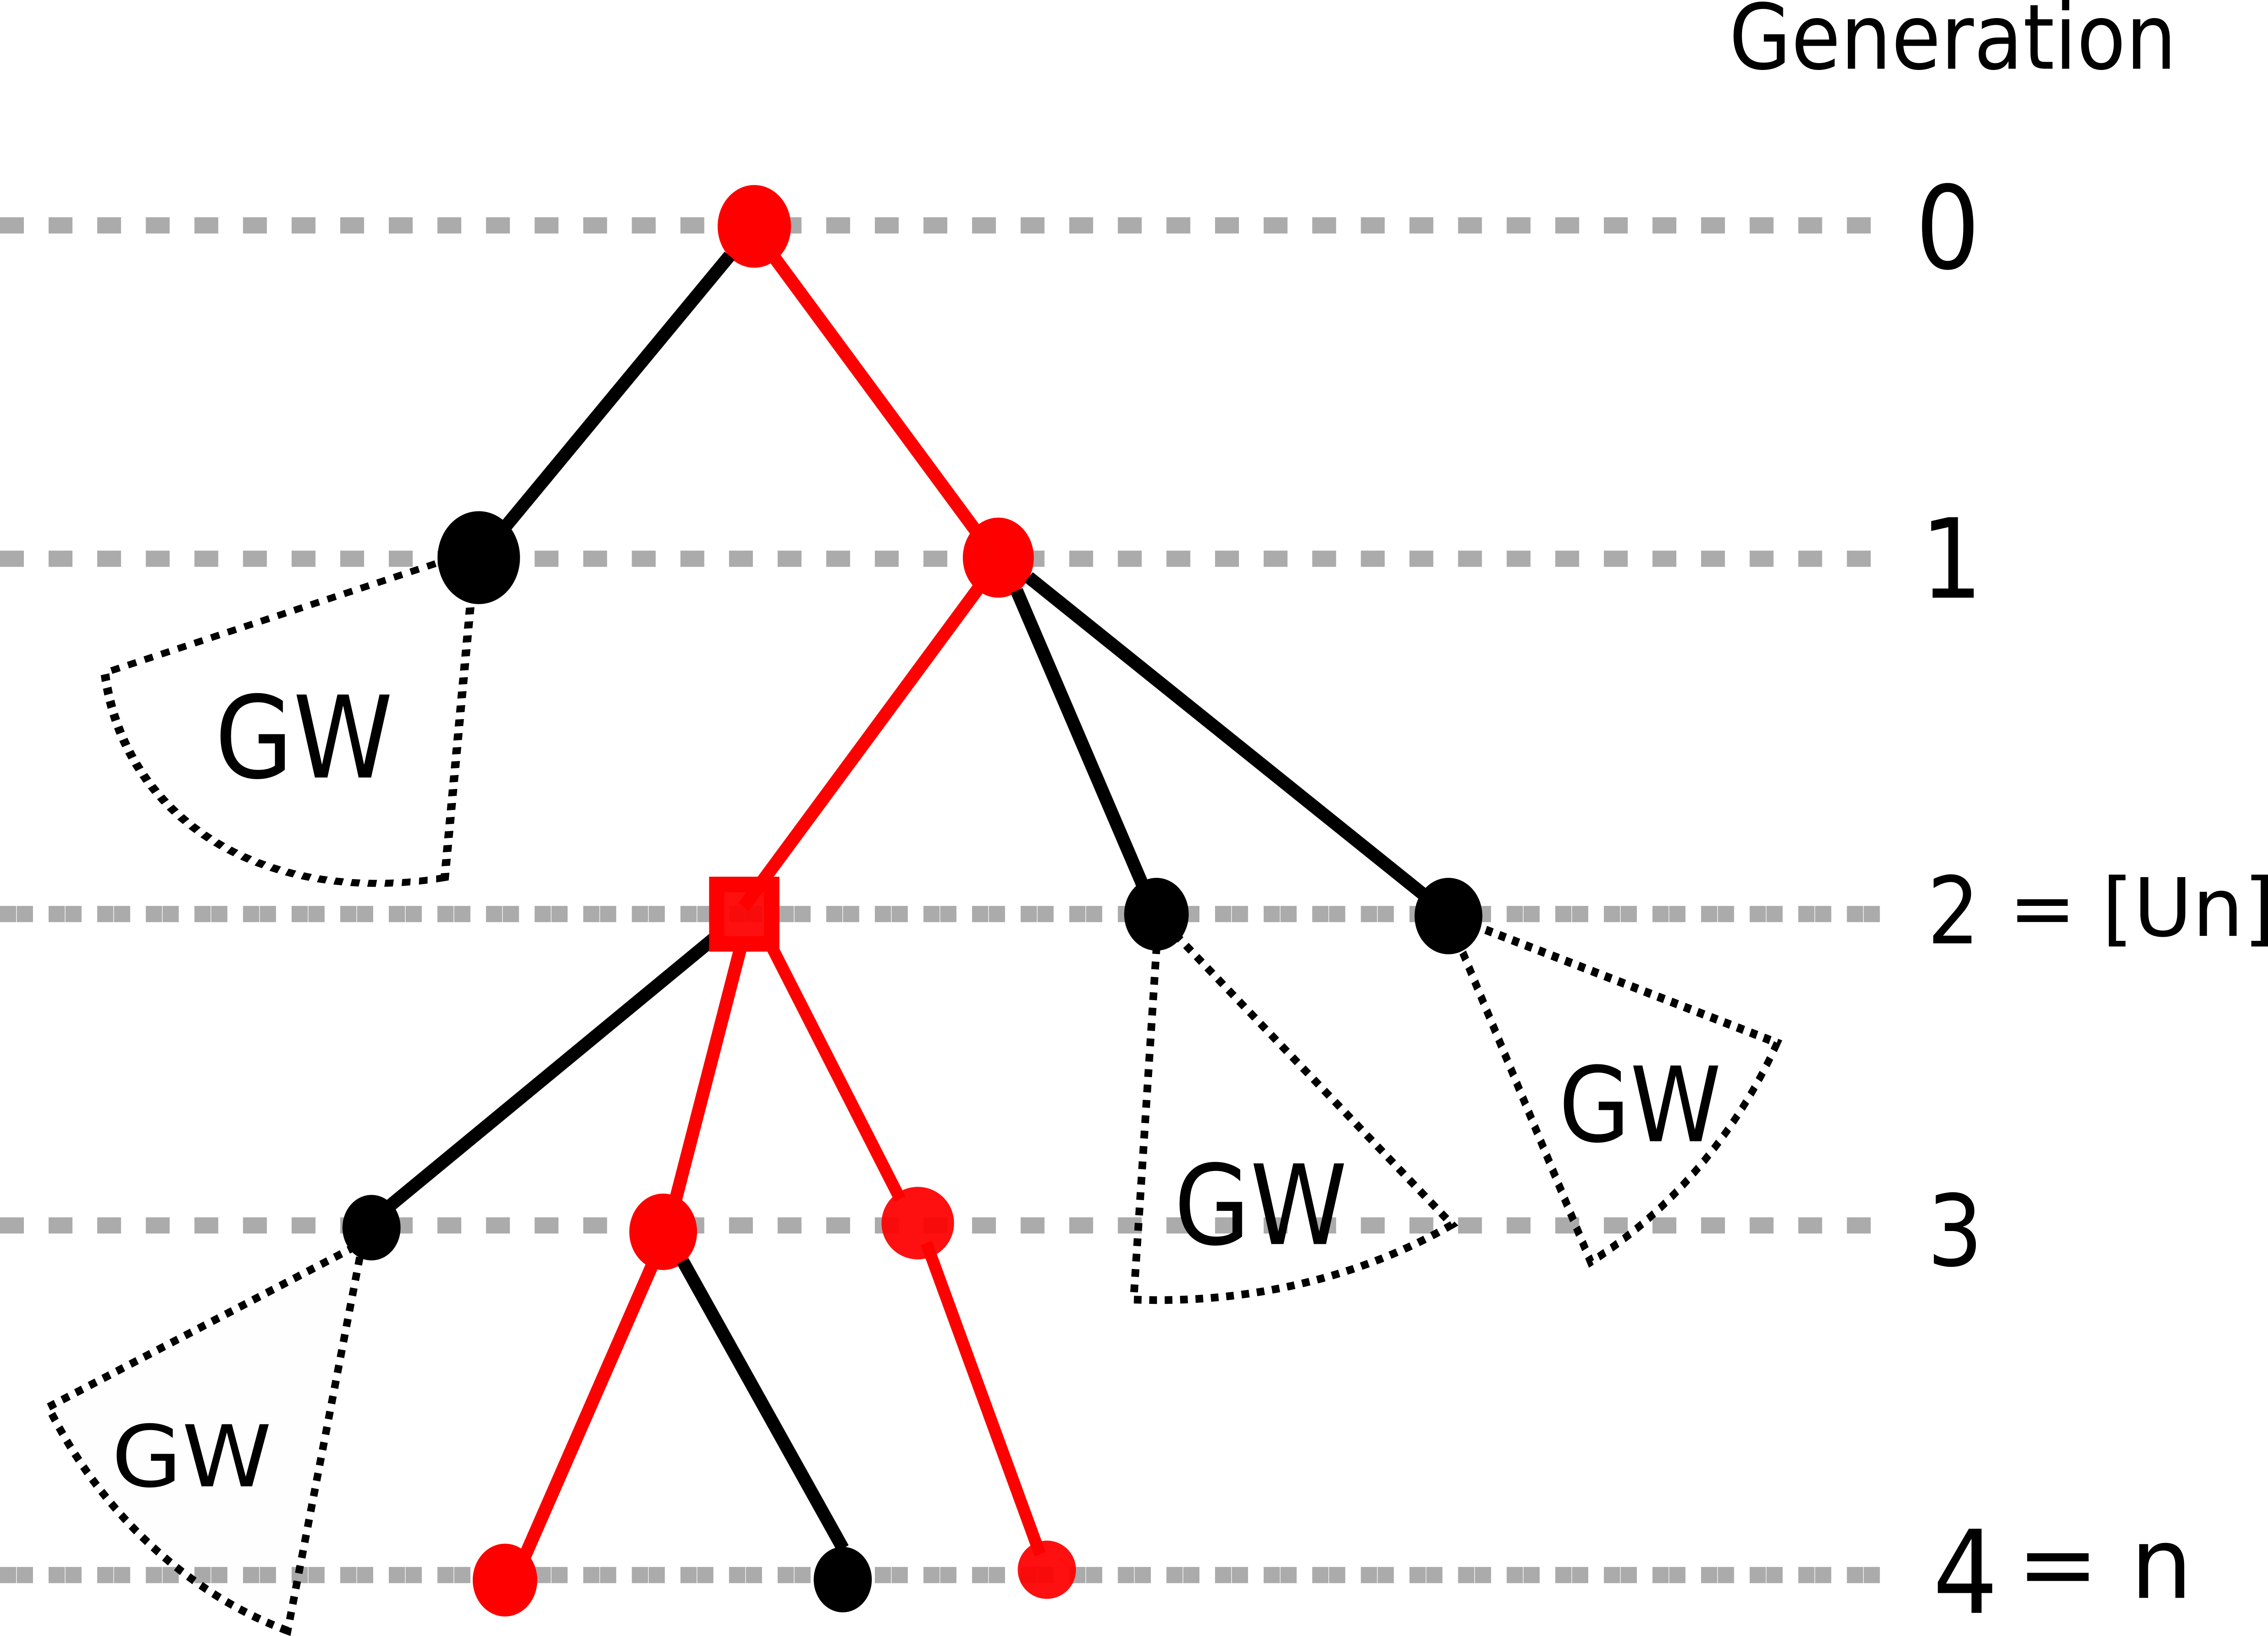
\includegraphics[scale=0.35]{2-spine.png}
  \end{tabular}
\end{figure}
Using this decomposition, we give a new probabilistic proof of Yaglom's theorem for critical Galton-Watson trees.
\end{frame}
\begin{frame}{Other Results}
In chapter 4, we proof the following:
\begin{block}{Theorem 4.}
  Suppose that $(X_t)_{t\geq \infty}$ is a non-persistent superprocess, i.e. $\mathbf P_{\delta_x}(\|X_t\| = 0) >0$ for each $x\in E$ and $t>0$. Then for each $f\in b\mathscr B_E$, the map $(t,x) \mapsto U_tf(x)$ given by
  \begin{align}
    e^{U_t( f)(x)} = \mathbf P_{\delta_x}[e^{i X_t(f)}]
  \end{align}
is the solution of the following equation:
\begin{align}
  U_tf(x) - \Pi_{x}\left[ \int_0^t \psi\left(\xi_s, - U_{t-s} f(\xi_s)\right) ds \right]
= i \Pi_x[f(\xi_t)], \quad t\geq 0, x\in E.
\end{align}
\end{block}
This result characterize the distribution of $X_t(f)$ where the testing function $f$ can take both positive and negative values.
\end{frame}

\section{References}
\begin{frame}
\frametitle<presentation>{References}
    
My Ph.D. thesis is based on the following works:
\begin{thebibliography}{10} 
    
\beamertemplatearticlebibitems
  
  \bibitem{RenSongSun2017A-2-spine}
  Ren, Y.-X., Song, R. and Sun, Z.:
  \emph{A 2-spine decomposition of the critical Galton-Watson tree and a probabilistic proof of Yaglom's theorem.}
  Electron. Commun. Probab. 23 (2018), Paper No. 42, 12 pp.
 
  \bibitem{RenSongSun2017Spine}
  Ren, Y.-X., Song, R. and Sun, Z.:
  \emph{Spine decompositions and limit theorems for a class of critical superprocesses.}
  Acta Appl. Math. (2019), https://doi.org/10.1007/s10440-019-00243-7

  \bibitem{RenSongSun2018Limit}
  Ren, Y.-X., Song, R. and Sun, Z.:
  \emph{Limit theorems for a class of critical superprocesses with stable branching.} ArXiv:1807.02837

  \bibitem{RenSongSun2019Stable}
    Ren, Y.-X., Song, R., Sun, Z. and Zhao, J.:
    \emph{Stable Central Limit Theorems for Super Ornstein-Uhlenbeck processes.}
    ArXiv:1903.03751

  \end{thebibliography}
\end{frame}

\begin{frame}
  \centering \Large
  \emph{感谢!}
\end{frame}

\end{document}

\begin{comment}
\begin{frame}[allowframebreaks]
\frametitle<presentation>{References}
    
\begin{thebibliography}{10} 
    
\beamertemplatearticlebibitems

\bibitem{AsmussenHering1983Branching}
  Asmussen, S. and Hering, H.:
  \emph{Branching processes}.
  Progress in Probability and Statistics, 3.
  Birkh{\"a}user Boston, Inc., Boston, MA, 1983.
  
  \bibitem{AthreyaNey1974Functionals}
  Athreya, K.~B. and Ney, P.~E.:
  \emph{Functionals of critical multitype branching processes}.
  Ann. Probability \textbf{2} (1974), 339--343. \MR{0356264}
  
  \bibitem{AthreyaNey1972Branching}
  Athreya, K. and Ney, P.:
  \emph{Branching processes}.
  Die Grundlehren der mathematischen Wissenschaften, Band 196.
  Springer-Verlag, New York-Heidelberg, 1972.
  
  \bibitem{BinghamGoldieTeugels1989Regular}
  Bingham, N.~H., Goldie, C.~M. and Teugels J.~L.:
  \emph{Regular variation}.
  Encyclopedia of Mathematics and its Applications, 27.
  Cambridge University Press, Cambridge, 1989.
  
  \bibitem{Borovkov1989Method}
  Borovkov, K.~A.:
  \emph{A method for the proof of limit theorems for branching processes}.
  Teor. Veroyatnost. i Primenen. \textbf{33} (1988), no. 1, 115--123;
  translation in Theory Probab. Appl. \textbf{33} (1988), no. 1, 105–113.
  
  \bibitem{EckhoffKyprianouWinkel2015Spines}
  Eckhoff, M., Kyprianou, A.~E., Winkel, M.:
  \emph{Spines, skeletons and the strong law of large numbers for superdiffusions.}
  Ann. Probab. \textbf{43} (2015), no. 5, 2545–2610.
  
  \bibitem{EnglanderKyprianou2004Local}
  Engländer, J., Kyprianou, A.~E.:
  \emph{Local extinction versus local exponential growth for spatial branching processes.}
  Ann. Probab. \textbf{32} (2004), no. 1A, 78–99.
  
  \bibitem{EvansPerkins1990Measure-valued}
  Evans, S.~N., Perkins, E.:
  \emph{Measure-valued Markov branching processes conditioned on nonextinction.}
  Israel J. Math. \textbf{71} (1990), no. 3, 329–337.
  
  \bibitem{GoldsteinHoppe1978Critical}
  Goldstein, M.~I., Hoppe, F.~M.:
  \emph{Critical multitype branching processes with infinite variance.}
  J. Math. Anal. Appl. \textbf{65} (1978), no. 3, 675–686.
  
  \bibitem{Harris2002The-theory}
  Harris, T. E.:
  \emph{The theory of branching processes.}
  Die Grundlehren der Mathematischen Wissenschaften, Bd. 119 Springer-Verlag, Berlin; Prentice-Hall, Inc., Englewood Cliffs, N.J. 1963.
  
  \bibitem{IyerLegerPego2015Limit}
  Iyer, G., Leger, N., Pego, R.~L.:
  \emph{Limit theorems for Smoluchowski dynamics associated with critical continuous-state branching processes.}
  Ann. Appl. Probab. \textbf{25} (2015), no. 2, 675–713.
  
  \bibitem{JoffeSpitzer1967On-multitype}
  Joffe, A. and Spitzer, F.:
  \emph{On multitype branching processes with {$\rho \leq 1$}.}
  J. Math. Anal. Appl. \textbf{19} (1967), 409--430.
  
  \bibitem{KestenNeySpitzer1966The-Galton-Watson}
  Kesten, H., Ney, P. and Spitzer, F.:
  \emph{The {G}alton-{W}atson process with mean one and finite variance.}
  Teor. Verojatnost. i Primenen. \textbf{11} (1966), 579--611.
  
  \bibitem{KimSong2008Intrinsic}
  Kim, P. and Song, R.:
  \emph{Intrinsic ultracontractivity of non-symmetric diffusion semigroups in bounded domains.}
  Tohoku Math. J. (2) \textbf{60} (2008), no.~4, 527--547.
  
  \bibitem{Kolmogorov1938Zur-losung}
  Kolmogorov, A.~N.:
  \emph{Zur l{\"o}sung einer biologischen aufgabe.}
  Comm. Math. Mech. Chebyshev Univ. Tomsk \textbf{2} (1938), no.~1, 1--12.
  
  \bibitem{Kyprianou2014Fluctuations}
  Kyprianou, A.~E.:
  \emph{Fluctuations of Lévy processes with applications.}
  Introductory lectures. Second edition. Universitext. Springer, Heidelberg, 2014.
  
  \bibitem{Kyprianou2008Continuous}
  Kyprianou, A.~E., Pardo, J. C.:
  \emph{Continuous-state branching processes and self-similarity.}
  J. Appl. Probab. \text{45} (2008), no. 4, 1140–1160.

  \bibitem{Li2011Measure-valued}
  Li, Z.:
  \emph{Measure-valued branching {M}arkov processes.}
  Probability and its Applications (New York), Springer, Heidelberg, 2011.
  
  \bibitem{LiuRenSong2009Llog}
  Liu, R.-L., Ren, Y.-X. and Song, R.
  \emph{{$L\log L$} criterion for a class of superdiffusions.}
  J. Appl. Probab. \textbf{46} (2009), no.~2, 479--496.
  
  \bibitem{Pakes2010Critical}
  Pakes, A.~G.:
  \emph{Critical {M}arkov branching process limit theorems allowing infinite variance.}
  Adv. in Appl. Probab. \textbf{42} (2010), no.~2, 460--488.
  
  \bibitem{Powell2015An-invariance}
  Powell, E.:
  \emph{An invariance principle for branching diffusions in bounded domains.}
  arXiv:1512.00031
  
  \bibitem{RenSongSun2017A-2-spine}
  Ren, Y.-X., Song, R. and Sun, Z.:
  \emph{A 2-spine decomposition of the critical Galton-Watson tree and a probabilistic proof of Yaglom's theorem.}
  arXiv:1706.07125
  
  \bibitem{RenSongSun2017Spine}
  Ren, Y.-X., Song, R. and Sun, Z.:
  \emph{Spine decompositions and limit theorems for a class of critical superprocesses.}
  arXiv:1711.09188

  \bibitem{RenSongSun2018Limit}
  Ren, Y.-X., Song, R. and Sun, Z.:
  \emph{Limit theorems for a class of critical superprocesses with stable branching.} ArXiv:1807.02837
  
  \bibitem{RenSongZhang2015Limit}
  Ren, Y.-X., Song, R. and Zhang, R.:
  \emph{Limit theorems for some critical superprocesses.}
  Illinois J. Math. \textbf{59} (2015), no.~1, 235--276.
  
  \bibitem{RenSongZhang2017Central}
  Ren, Y.-X., Song, R. and Zhang, R.:
  \emph{Central limit theorems for supercritical branching nonsymmetric {M}arkov processes.}
  Ann. Probab. \textbf{45} (2017), no.~1, 564--623.
  
  \bibitem{RenYangZhao2014Conditional}
  Ren, Y.-X., Yang, T., Zhao, G.-H.:
  \emph{Conditional limit theorems for critical continuous-state branching processes.}
  Sci. China Math. \textbf{57} (2014), no. 12, 2577–2588.
  
  \bibitem{Schaefer1974Banach}
  Schaefer, H.~H.:
  \emph{Banach lattices and positive operators.}
  Die Grundlehren der mathematischen Wissenschaften, Band 215. Springer-Verlag, New York-Heidelberg, 1974.
  
  \bibitem{Slack1968A-branching}
  Slack, R.~S.:
  \emph{A branching process with mean one and possibly infinite variance.}
  Z. Wahrscheinlichkeitstheorie und Verw. Gebiete \textbf{9} (1968), 139--145.
  
  \bibitem{Slack1972Further}
  Slack, R.~S.: \emph{Further notes on branching processes with mean {$1$}.}
  Z. Wahrscheinlichkeitstheorie und Verw. Gebiete \textbf{25} (1972/73), 31–38.
  
  \bibitem{Vatutin1977Limit}
  Vatutin, V. A.:
  \emph{Limit theorems for critical multitype Markov branching processes with infinite second moments.}
  Mat. Sb. (N.S.) \textbf{103(145)} (1977), no. 2, 253–264, 319.
  
  \bibitem{Yaglom1947Certain}
  Yaglom, A. M.:
  \emph{Certain limit theorems of the theory of branching random processes.}
  Doklady Akad. Nauk SSSR (N.S.) \textbf{56} (1947). 795–798.
  
  \bibitem{Zolotarev1957More}
  Zolotarev, V. M.:
  \emph{More exact statements of several theorems in the theory of branching processes.}
  Teor. Veroyatnost. i Primenen. \txtbf{2} (1957), 256–266.

  \end{thebibliography}
\end{frame}
\end{comment}

\end{document}

%%% Local Variables: 
%%% TeX-engine: xetex
%%% End:
